\section{E-Assessment}


\subsection{Einleitung}
In der Hochschullehre nehmen Leistungs�berpr�fungen einen integralen Bestandteil in Lehr- und Lernprozessen ein. Ein Augenmerk liegt hierbei auf der Identifizierung und Bewertung individueller Lernfortschritte \cite[S. 23 f.]{Kuchen2010}. Darunter wird insbesondere das Pr�fen und Bewerten einzelner �bungen als Teil einer p�dagogischen Handlungseinheit verstanden. Dabei k�nnen die verschiedenen �bungsphasen und -iterationen unterschiedliche L�ngen haben und inhaltliche Abh�ngigkeiten haben \cite[S. 25]{Kuchen2010}. Abbildung \ref{fig:Uebungsbetrieb} zeigt den Lehr-Lern-Prozess eines �bungsbetriebs.

\begin{figure}[htbp] 
  \centering
     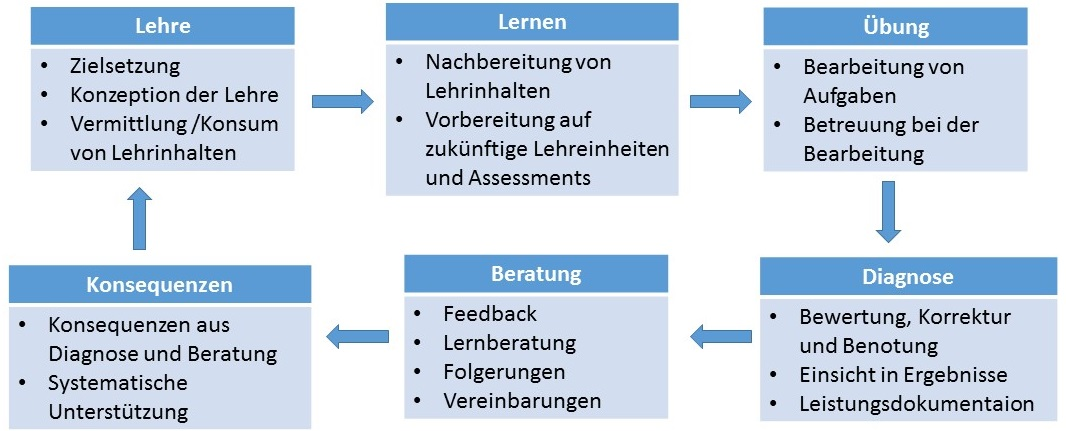
\includegraphics[width=0.9\textwidth]{graphics/Uebungsbetrieb.jpg}
  \caption{Iterative Lehr-Lern-Prozesse eines �bungsbetriebs}
  \label{fig:Uebungsbetrieb}
\end{figure} 

Im Regelfall beginnt ein �bungszyklus mit der Phase der Lehre. In dieser Phase vermittelt der Lehrende dem Studierenden die entsprechenden Inhalte. Anschlie�end hat der Studierende in der Lernphase die M�glichkeit das vermittelte Wissen im Selbststudium zu vertiefen. In einer darauf folgenden �bung kann der Studierende sein theoretisches Wissen anhand geeigneter praktischer �bungen ausprobieren und festigen. Im Anschluss folgt die Diagnose der �bung, welche Korrektur und Benotung beinhaltet. Dies geschieht im Regelfall durch DozentInnen oder TutorInnen, kann aber auch durch KommilitonInnen erfolgen (Peer Review). Es sollte ein Feedback �ber die erbrachte Leistung und Ratschl�ge folgen. Optional kann aus den Ratschl�gen eine Leistungsvereinbarung abgeleitet werden \cite[S. 25 f.]{Kuchen2010}.

Auf Grund des Bologna-Prozesses, Sparma�nahmen, Diskussionen �ber die Verwendung von Studiengeb�hren und steigende Studierendenzahlen wird im Bereich der �bungsangebote der Einsatz von E-Assessments vermehrt in Betracht gezogen \cite[S. 9]{kortemeyer2010}. 
Unter e-Assessment versteht man das Spektrum der auf den neuen (elektronischen) IKT basierenden Verfahren der lehrzielbezogenen Bestimmung, Beurteilung, Bewertung, Dokumentation und R�ckmeldung der jeweiligen Lernvoraussetzungen, des aktuellen Lernstandes oder der erreichten Lernergebnisse/ -leistungen vor, w�hrend (?Assessment f�r das Lernen?) oder nach Abschluss (?Assessment des Lernens?) einer spezifischen Lehr-Lernperiode \cite[S. 6]{Bloh2006}. E-Assessment-Systeme k�nnen des Weiteren Nutzen f�r Lehrende und Lernende bieten. Cook und Jenkins identifizierten neuen Vorteile. Bei den Wichtigsten handelt es sich um die M�glichkeiten des direkten Feedbacks und der sofortigen und objektiven Benotung.  Au�erdem bieten E-Assessment-Systeme einfache Skalierbarkeit und Wiederverwendbarkeit \cite[S. 3]{Cook2010}. E-Assessments k�nnen hinsichtlich ihrer Hauptaufgabe in drei Typen unterteilt werden \cite[S. 8]{Cook2010}:
\begin{itemize}
\item \textbf{Diagnostische Assessments} finden normalerweise zu beginn einer Lehrveranstaltung statt um m�gliche Wissensl�cken bei Teilnehmern aufzudecken und gegebenenfalls ein Nachbesserungsangebot zu schaffen. 
\item \textbf{Formative Assessments} erm�glicht Studierenden und Lehrenden einen �berblick �ber den aktuellen Lernstand zu erhalten. E-Assessment erm�glicht Studierenden weiterhin ein direktes Feedback.
\item \textbf{Summative Assessments} bieten eine Bewertungsgrundlage �ber den Lernfortschritt eines Studierenden. Bei diesem Typen steht im Gegensatz des Feedbacks die Notengebung im Vordergrund.
\end{itemize}

Leistung�berpr�fungen sind ein integraler Bestandteil der Lehr- und Lernprozesse. \cite{Kuchen2010}. 

W�chentliche �bungszettel --> theoretisch erlerntes Wissen durch Bearbeitung geeigneter Aufgaben reflektieren und verinnerlichen S.24



\subsection{Das E-Assessment-System EASy der WWU M�nster}